\documentclass[a4paper,12pt]{article}
\usepackage[english,russian]{babel}
\usepackage[utf8]{inputenc}
\usepackage{latexsym,mathrsfs}
\usepackage{stmaryrd, enumitem}
\usepackage{amsthm,amsfonts,amssymb,amsmath}
\usepackage{geometry}
\usepackage{tempora}
\usepackage{graphicx}
\usepackage{url}

\geometry{top=17mm}  \geometry{bottom=20mm}
\geometry{left=17mm} \geometry{right=17mm}
\linespread{1.1}
\parindent=5mm

\def\titleK#1{\begin{center}{\Large\textbf{#1}}\end{center}}
\def\authorK#1{\begin{center}{#1}\end{center}}

\newenvironment{abstractK}{}

\newtheorem{theorem}{Теорема}
\newtheorem{lemma}{Лемма}
\newtheorem{corollary}{Следствие}
\newtheorem{proposition}{Предложение}
\newtheorem{statement}{Утверждение}
\theoremstyle{definition}
\newtheorem{definition}{Определение}
\newtheorem{problem}{Задача}
\newtheorem{question}{Вопрос}
\newtheorem{conjecture}{Гипотеза}
\newtheorem{construction}{Конструкция}
\newtheorem{remark}{Замечание}

%ВАЖНО: Просьба пользоваться имеющимися окражениями-теоремами
%ВАЖНО: Не менять и не добавлять ничего выше этой строки.
%Изменения вносить только внутри окружения \begin{document}\end{document}

\begin{document}

%Название доклада
\titleK{Исследование аппаратно-программных реализаций алгоритмов защиты информации}

%Информация об авторах (ЗАМЕНИТЕ на свои данные)
\authorK{Д.~С.~Соловьёв$^{1}$, А.~В.~Тюндин$^{2}$\\
$^{1}$Южный федеральный университет \\ $^{2}$НГТУ им. Р. Е. Алексеева \\ 
{\bf E-mail:} dsolove@sfedu.ru, AlexanderTyundin@yandex.ru}

\begin{abstract}

\end{abstract}


{\bf Актуальность:} Проект направлен на изучение методов реализаций широко распространенных алгоритмов криптографической защиты информации; изучение алгоритмов защиты от статического и динамического анализа, а также на развитие у исследователя нестандартного подхода к анализу надежности механизмов защиты.

{\bf Ключевые слова:} \textit{проверка надежности системы защиты исполняемого кода, статический и динамический анализ, информационная безопасность.} 


\begin{abstractK}

\section*{Введение}

В условиях стремительного развития информационных технологий и повсеместной цифровизации всё больше критически важных функций реализуется в программном обеспечении. Это делает программные продукты привлекательной целью для злоумышленников, стремящихся получить несанкционированный доступ к алгоритмам и бизнес-логике приложения. Конкретные программные реализации алгоритмов, в настоящее время, все чаще составляют коммерческую тайну. Таким образом, конкретная реализация программного продукта также является данными, утрата которых может нанести чувствительный финансовый и репутационный ущерб коммерческой компании.

Наиболее действенными инструментами в арсенале нарушителей при исследовании программного продукта остаются методы статического и динамического анализа, позволяющие восстановить чувствительные элементы логики приложения и бизнес-процесса.

Современные средства анализа – от дизассемблеров и отладчиков до систем автоматизированного анализа программной реализации становятся всё более доступными и мощными. Это значительно снижает порог входа для злоумышленников и делает традиционные подходы к защите, такие как простая обфускация или упаковка исполняемых файлов, недостаточно эффективными. Настоящая работа представляет обзор и оценку применимости широко распространенных методов зашщиты исполняемого кода.


\section*{Цель исследования:}
Целью исследования является 

\section*{Задачи исследования:}
\begin{enumerate}
	\item Обзор современных алгоритмов  защиты от статического и динамического анализа;
	\item Исследование конкретной реализации алгоритмов защиты от статического и динамического анализа;
    \item Исследование алгоритмов поиска реализаций широко распространенных методов криптографической защиты информации;
\end{enumerate}

\section*{Объект исследования}



\section*{2. ВАША СОДЕРЖАТЕЛЬНАЯ ЧАСТЬ}


\section*{Заключение}

ПЕРЕПИСАТЬ



\end{abstractK}

\renewcommand\refname{\center \textnormal{\normalsize{ЛИТЕРАТУРА}}}
%Список литературы
\begin{thebibliography}{}
ВСТАВИТЬ БИБЛИОГРАФИЮ ИЗ ТЕКСТОВОГО ФАЙЛА
\end{thebibliography}

\bf{Кураторы исследования:} \rm{\\
 Яковлев Александр Андреевич~--- преподаватель 41 кафедры НИЯУ МИФИ;
 
\end{document}


% Пример вставки картинок
\begin{figure}[h]
\begin{minipage}[h]{0.49\linewidth}
\center{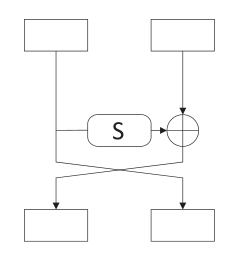
\includegraphics[width=1\linewidth]{feistel.png} }
\caption{Сеть Фейстеля}
\label{fig:image1}
\end{minipage}
\hfill
\begin{minipage}[h]{0.49\linewidth}
\center{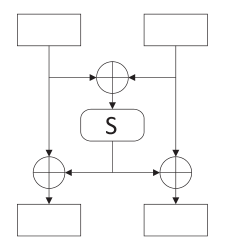
\includegraphics[width=1\linewidth]{laimassey.png} }
\caption{Схема Лая--Месси}
\label{fig:image2}
\end{minipage}
\end{figure}

\newpage
Вставка одиночного рисунка в центре: 

\begin{figure}[h]
\center{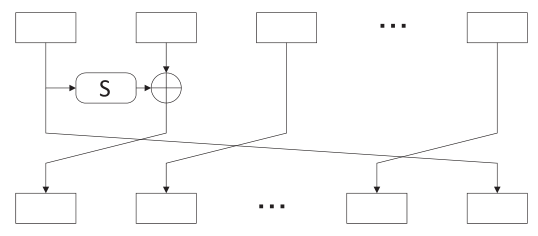
\includegraphics{gfn1.png}}
\caption{Еще схема}
\label{fig:pic3}
\end{figure}

В таблице~\ref{table:cryptosystem} приведены...

\begin{table}[h]
\centering
\begin{tabular}{|c|c|}
\hline
RSA & параметры 1\\
\hline
Classic McEliece & параметры 2\\
\hline
\end{tabular}
\caption{Параметры криптосистемы}
\label{table:cryptosystem}
\end{table}